\section{Evaluation}
\label{sec:result}

\begin{table}[b]
	\centering
	\caption{Absolute Trajectory Error for ViViD sequences}
	\resizebox{0.8\columnwidth}{!}{%
		\begin{tabular}{|c|c|c|}
			\hline
			Sequence           & ORB2         & Ours       \\ \hline
			Robust\_Global     & 0.0726       & 0.1024     \\ \hline
			Unstable\_Global   & 0.1625       & 0.3748     \\ \hline
			Aggressive\_Global & Track lost   & 0.3781     \\ \hline
			Robust\_Dark       & Init fail    & 0.2563     \\ \hline
			Unstable\_Dark     & Init fail    & 0.4041     \\ \hline
			Aggressive\_Dark   & Init fail    & 0.6108     \\ \hline
		\end{tabular}%
	}
	\label{tab:errmat}
\end{table}

We evaluate our algorithm along ViViD indoor sequences. Since we aim for robust trajectory
estimation even under aggressive motion and dynamic lighting, evaluation sequences included
the variances. We calculated absolute trajectory error for each sequences and compared against
ORB-SLAM2 \cite{mur2017orb}, using RGB-D configuration. 
The absolute trajectory error of sequences are listed in \tabref{tab:errmat}. ORB-SLAM2 shows
desirable performance for robust environments, but fails on aggressive motion and dark scenes.

The DAVIS camera produces events from 240$\times$180 pixel array, asynchronously at a
timing when the luminescence value of the pixel changes. Therefore, it provides high dynamic
range to cover large range of lighting conditions. Since ORB-SLAM2 is based on image features,
it ORB-SLAM2 fails to complete estimating the whole trajectory except robust motion and modest
lighting conditions. However, our sensor configuration does not fails on given sequences.

%FIGURE
\begin{figure*}[t]
	\centering
	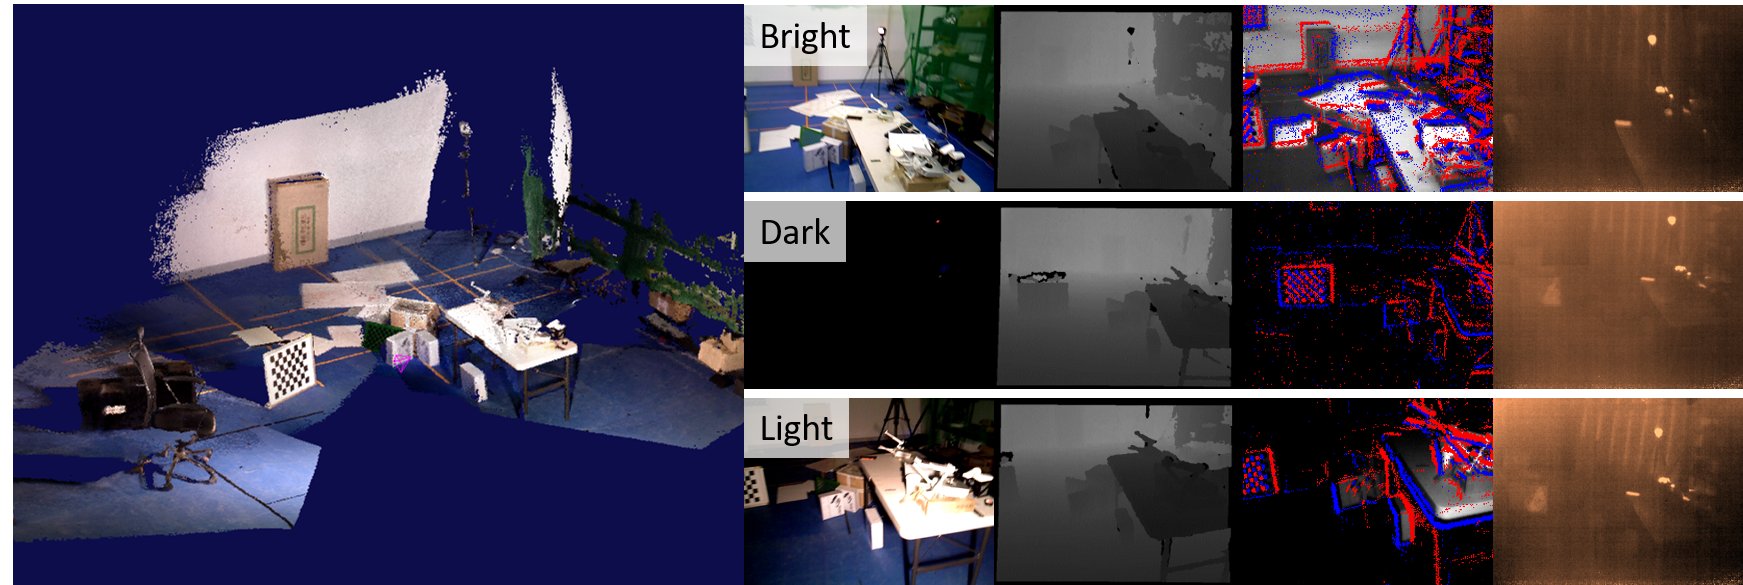
\includegraphics[width=0.875\textwidth]{figures/indoor_samples_with_map}
	
	\caption{Scene overview of Vision for Visibility Dataset (left), with data sample from each sensors (right).
		Images acquired from each sensors are illustrated for each lighting conditions, listed left from
		RGB, depth, events, thermal camera.
	}
	
	\label{fig:samplesequence}
\end{figure*}


%FIGURE
\begin{figure*}[!t]
	\centering
	\includegraphics[width=0.86\textwidth]{figures/fig3}
	
	\caption{Estimated trajectory and reconstructed pointcloud for vivid dataset, for varying light sequence.
		As there is lighting change over time, image feature based ORB-SLAM2 (red path) fails to estimate trajectory
		when the light turns off. However, Ours (green path) succeeds on estimating the trajectory robustly under
		circumstances.}
	
	\label{fig:trajsample}
\end{figure*}


Since the resolution of DAVIS camera is relatively lower than other sensors, the output
of our algorithm does not gives better results to ORB-SLAM2, on stable environments.
In global lighting sequences the room was sufficiently bright with constant ambient
light. And for the dark and local light sequences, we ran our experiment with the
ambient light turned off. In local light sequences, only an LED installed with sensor
rig was turned on, producing unequally configured lighting profile for the scene.
As in \figref{fig:trajsample} local light source changes its brightness, and RGB-based
features fail easily, yielding tracking lost.
